% Use only LaTeX2e, calling the article.cls class and 12-point type.

\documentclass[12pt]{article}
\usepackage{graphicx}
\graphicspath{ {./Users/petertran/Desktop} }

% Users of the {thebibliography} environment or BibTeX should use the
% scicite.sty package, downloadable from *Science* at
% http://www.sciencemag.org/authors/preparing-manuscripts-using-latex 
% This package should properly format in-text
% reference calls and reference-list numbers.

\usepackage{scicite}

\usepackage{times}

\usepackage{enumitem}

\usepackage{amsmath}

\usepackage{tikz}

\usetikzlibrary{shapes.geometric, arrows}

\usetikzlibrary{positioning}

\usepackage{pgfplots}

\usepackage{fontawesome5}

\usepackage{hyperref}

\usepackage{graphicx}

\usepackage{graphicx,calc}
\newlength\myheight
\newlength\mydepth
\settototalheight\myheight{Xygp}
\settodepth\mydepth{Xygp}


\tikzstyle{process} = [rectangle, minimum width=3cm, minimum height=1cm, text centered, draw=black, fill=orange!30]

\tikzstyle{decision} = [diamond, minimum width=3cm, minimum height=1cm, text centered, draw=black, fill=green!30]


\tikzstyle{arrow} = [thick,->,>=stealth]



% The preamble here sets up a lot of new/revised commands and
% environments.  It's annoying, but please do *not* try to strip these
% out into a separate .sty file (which could lead to the loss of some
% information when we convert the file to other formats).  Instead, keep
% them in the preamble of your main LaTeX source file.


% The following parameters seem to provide a reasonable page setup.

\topmargin 0.0cm
\oddsidemargin 0.2cm
\textwidth 16cm 
\textheight 21cm
\footskip 1.0cm


%The next command sets up an environment for the abstract to your paper.

\newenvironment{sciabstract}{%
\begin{quote} \bf}
{\end{quote}}



% Include your paper's title here

\title{SolBunny Hop-paper \\ {\it into the nom\/} } 


% Place the author information here.  Please hand-code the contact
% information and notecalls; do *not* use \footnote commands.  Let the
% author contact information appear immediately below the author names
% as shown.  We would also prefer that you don't change the type-size
% settings shown here.

\author
{271077$^{1\ast}$, KJ$^{1}$, BunnyHunter$^{1}$, Corporate Panda$^{1}$, myxilplix$^{1}$, bunnyclock$^{1}$, \\
Systematic3x$^{1}$, cedarandsmoke$^{1}$, GRACKATTACK$^{1,2}$, gerald hefner$^{1,2}$\\
\\
\normalsize{$^{1}$Department of Anomalous Bunnynomics, University of SolBunny,}\\
\normalsize{SolBunny Street, SolTown, SBM 1337, Moon}\\
\\
\normalsize{$^{2}$Supreme leaders at The University of SolBunny}\\
\\
\normalsize{$^\ast$To whom correspondence should be addressed; E-mail: Bunnynomics101@gmail.com}\\
\normalsize{ \raisebox{-.9\mydepth}{
\includegraphics[height=+1.2\myheight]{solbunny}} \href{https://solbunny.io}{SolBunny} $\vert$ \faIcon{github} \href{https://github.com/BunnyNomics101}{Github} $\vert$ \faIcon{twitter} \href{https://twitter.com/SolanaBunny}{Twitter} $\vert$ \faIcon{discord} \href{https://discord.gg/Pz5q9xeP} {Discord} 
$\vert$ \faIcon{reddit} \href{https://www.reddit.com/r/SolBunny/}{Reddit}}
\\
\date{\today}
}

% Include the date command, but leave its argument blank.

\date{}




%%%%%%%%%%%%%%%%% END OF PREAMBLE %%%%%%%%%%%%%%%%



\begin{document} 

% Double-space the manuscript.

\baselineskip24pt

% Make the title.

\maketitle 



% Place your abstract within the special {sciabstract} environment.

\begin{sciabstract}
  This hop-paper serves as a whitepaper for the {\it SolBunny metaDAO (SBm)\/}, and describe the vision of the ecosystem. 
  SBm is presented as a new form of DAO, metaDAO, based on liquid democracy with the capacity to run a decentralized exchange.
  In addition, the protocol remains completely decentralized and autonomous despite a high complexity of connected applications. 
 The new era of metaDAOs will allow its users more control over their financial situation, both on-chain and in real-word situations.
\end{sciabstract}

% In setting up this template for *Science* papers, we've used both
% the \section* command and the \paragraph* command for topical
% divisions.  Which you use will of course depend on the type of paper
% you're writing.  Review Articles tend to have displayed headings, for
% which \section* is more appropriate; Research Articles, when they have
% formal topical divisions at all, tend to signal them with bold text
% that runs into the paragraph, for which \paragraph* is the right
% choice.  Either way, use the asterisk (*) modifier, as shown, to
% suppress numbering.

\section*{Introduction}

Modern society continues to advance and mature at a fast pace, enabling great possibilities. However, along with these enhancements come an increasing bureaucracy,  with inefficient and often slow systems, leading to an overload of pseudowork \cite{pseudowork}. Two important pillars suffer under these circumstances: democracy and economy. 

Western democracy today, meaning ‘rule of the people’, shares a close resemblance to Classical Athens \cite{ClassicalAthens} where people would gather around in meetings of the assembly or ecclesia. None of the assembly’s members were elected, and thus, greek democracy was open for any adult male over the age of 20 \cite{directDemocracy}. But direct democracy was not very scalable to modern society with more complex problems across multiple nations. Thus, the all-knowing voter who is active in all votings does not exist. In its place, most contemporary democracies are instead Democratic Republics, which use elected representatives who are supposed to vote in representation of the people's wishes. However, the current system is a blunt approximation which can often result in representatives acting in conflict to the interests of those whom they represent. Today’s representatives are in one way disconnected from their voters while at best, they are not able to accommodate the interests of all their constituents. 

The friction in western democracy reflects poorly in the economy as seen in the past decades, from financial crisis \cite{financialCrisis} to scandals \cite{panama, pandora}. The economics' decisions have become centralized into aristocratic ‘rule of the best’, and not intended for or reflect the best interest of society. A centralized allocation of resources (or money) is fallible, as influence accrues to a highly biased and often closed small social circle—thus, a reflexive social system hampers a thriving society \cite{reflexivity}. In the end, resources are wasted and/or concentrated into a minority.

SolBunny meta aims to challenge the status quo of aristocracy, and disrupt the current power-relationships by providing bona fide democracy. Subsequently, better decisions will be made for allocation of resources which represent people’s true value. There are three components in Solbunny metaDAO designed to achieve its vision: a immutable ledger, a voting system based on liquid democracy, and decentralized finance.


\section*{Immutable Ledger}

Trust is the foundation of every successful interaction, and in the event of discrepancy between parties, the objective truth should be retrievable from a track-record. Also, this track-record must be spatio-temporally preserved throughout history (who voted what and when). The blockchain, Solana \cite{SolanaWhitepaper}, offers a great solution to the needs of Solbunny by combining proof-of-stake (PoS) with proof-of-history (PoH) \cite{solanaIntro}. Briefly, PoS ensures a consensus between a set of independent entities while PoH maintains trustless synchronization by running an iterative SHA-256 hash function a certain number of times. Thus, a timestamp in history is not referred to as time in SI-units though it resembles the oscillations of caesium-133 in an atomic clock. Solbunny is based on Solana for exactly these reasons stated above, but a deeper understanding is beyond the scope of this article. The underlying technology of Solana are perfectly suitable for the vision of SolBunny, and the services of its metaDAO for community members. However, accessibility can still be censored at certain focal points such as web3 login, websites and APIs. One approach is to use the Arweave protocol \cite{arweave}. On top of its protocol layer is the ‘permaweb’: a permanent, decentralized, and resilient storage. Combining Polkadot’s heterogeneous multi-chain framework \cite{polkadot} with Arweave will ultimately grant SolBunny the ability to be an omnipresent system for the people by the people.

\section*{Liquid Democracy}
Democracy has a long history and has changed tremendously in a short period of time. However, SolBunny believes it's possible to bring democracy back to its roots—or to the so-called ‘rule of the people’. The principle of liquid democracy was first introduced in Sweden by a pirate party, and has since spread to over 40 NGOs including parliaments \cite{liquidDemocracy}. Liquid democracy, sometimes denoted delegative democracy or proxy voting, comes closest to the ideal of complete direct democracy \cite{id1, steffenGanghof}. The basic model for liquid democracy combines collective decision-making with flexible representatives that satisfy a reasonable participatory model and entitles the voter to the following:

\begin{enumerate}

\item Direct democratic component: Directly vote on all policy issues

\item Flexible delegation component: Delegate their votes to a representative

\begin{enumerate}
    \item On a singular issue
    \item On all policies in one area
    \item On all policies in all areas
  \end{enumerate}

\item Meta-delegation component: Representatives can delegate their votes to other representatives

\item Instant recall component: Terminate/revoke the delegation of their votes at any time

\end{enumerate}

Consider the following example of Chad and Wojak on Solana with SolBunny metaDAO: Both Chad and Wojak have two votes, vote A and vote B, to vote on STEM and/or humanities, respectively. One day SolBunny sets up a vote on both categories, STEM wants 2$\%$ of the treasury to expand its DeFi capacity while humanities wants 1$\%$ to buy some research articles for marketing. Chad thinks the metaDAO is not doing enough for DeFi so he casts both votes, through his wallet address, on STEM. In contrast, Wojak is uncertain on economics and decides to delegate his vote to Chad (now the representative) while his other vote goes to humanities. Chad then convinces Wojak to revoke his vote from humanities and delegate it to him. In the end, Chad has two more votes to DeFi, and all votes return to the last representative after voting has ended. However, Wojak can retrieve his votes from Chad at any time since he is the only one who possesses his original wallet address (Fig.1). \\

Figure 1: Liquid democracy\\

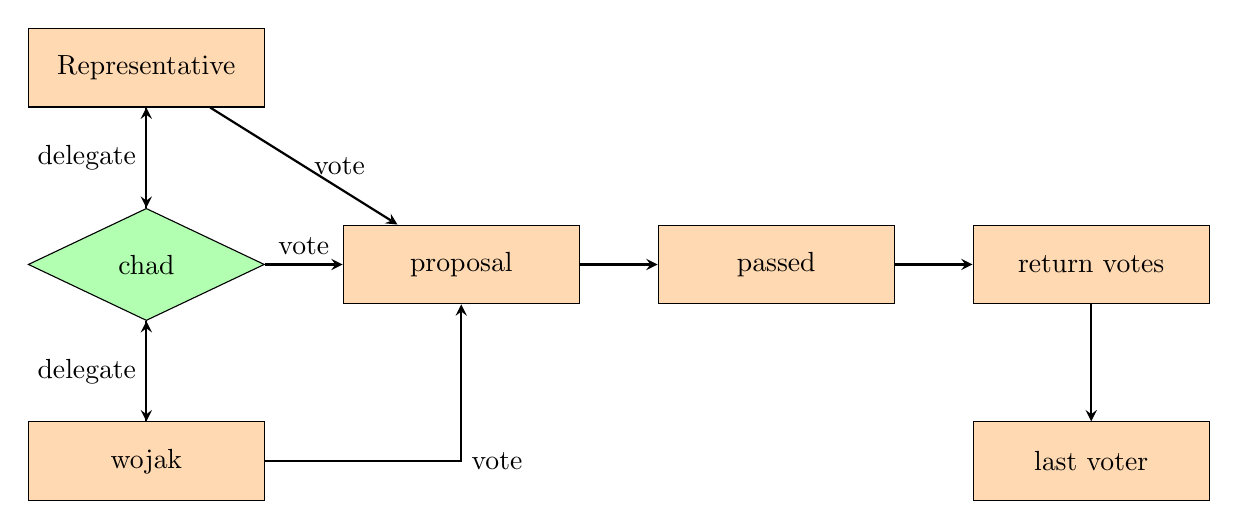
\begin{tikzpicture}[node distance=2cm]

\node (pro1) [process] {Representative};

\node (dec1) [decision, below of=pro1, yshift=-0.5cm] {chad};

\node (pro2) [process, right of=dec1, xshift=2cm] {proposal};

\node (pro3) [process, below of=dec1, yshift=-0.5cm] {wojak};

\node (pro4) [process, right of=pro2, xshift=2cm] {passed};

\node (pro5) [process, right of=pro4, xshift=2cm] {return votes};

\node (pro6) [process, below of=pro5, yshift=-0.5cm] {last voter};


\draw [arrow] (dec1) -- node[anchor=east] {delegate} (pro1);
\draw [arrow] (dec1) -- node[anchor=south] {vote} (pro2);
\draw [arrow] (pro3) -- node[anchor=east] {delegate} (dec1);
\draw [arrow] (pro3) -| node[anchor=west] {vote} (pro2);
\draw [arrow] (pro1) -- node[anchor=west] {vote} (pro2);
\draw [arrow] (pro1) -- (dec1);
\draw [arrow] (dec1) -- (pro3);
\draw [arrow] (pro2) -- (pro4);
\draw [arrow] (pro4) -- (pro5);
\draw [arrow] (pro5) -- (pro6);


\end{tikzpicture}

As the ecosystem expands, more and more subcategories can be voted on. Also, the members will gain popularity points in layer 2 of liquid democracy to be used as weighted votes. Popularity points can be achieved through other members independent of the voting systems, and some ways include (but not limited to): Contribution, personality, seniority, etc. There are infinite possibilities of how allocated points are translated into weighted votes, but the essential part is to not let one parameter dominate the individual voting-power. 

A governance-model on the blockchain is called a DAO (decentralized autonomous organisation) \cite{dao}, and often entails two tokens: One for the underlying governance, and another for supporting the ecosystem directly. DAOs are socio-technical ecosystems of mutually dependent parties where ‘Code is Constitution’, but most are far from autonomous. Instead, several central actors act as gatekeepers to reintroduce trust in a trustless environment. The problem occurs when a DAO (e.g. Tezos, DFINITY or Olympus) tries to adapt in a quickly ever-changing industry while still maintaining constitutional law of code ex-ante \cite{tezos}. Another pain-point is quorum-based voting because the threshold is arbitrarily chosen or a holographic consensus (e.g. DXdao and NecDAO) \cite{holo}; both are vulnerable to attack vectors and whale dominance.

SolBunny proposes a new model for DAOs called ‘metaDAO’, and uses liquid democracy as the center of its ecosystem. In the example above with Chad and Wojak, the originality of each individual is always preserved through their wallet address. And should a wallet be lost or given to another, a program could accept or reject the wallet based on votings. The practical implementation of liquid democracy in metaDAOs makes it inherently different from traditional DAOs on three levels:

\begin{enumerate}

\item There are centralized focal points or gatekeepers so fluidity is truly preserved

\item Does not enforce any arbitrary threshold other than what is decided on

\item It is both horizontally (voter to voter) and vertically (voter to system) flexible

\end{enumerate}

The term ‘meta’ refers to the metaverse \cite{metaverse} in digital transformation, but goes beyond its original definition. The metaverse will allow individuals to become their own unique reflection in a parallel universe, and best of all, they can be rewarded for their contribution. In SolBunny, this translates into special NFTs based on the level of contribution ultimately decided by its community members. More often than not, people are rewarded poorly if not at all for their contribution to a community. And while online forums such as Reddit \cite{reddit} provide a sense of affiliation, the reflection in real-life remains poor. NFT-awards/badges will play a tremendous role in SolBunny as they can act as reliable representatives of the ecosystem, bridging from blockchains to real-world actions. For example, certain NFT badges will allow its owners to increase the likelihood of a project being accepted into the SolBunny dex launchpad.

\section*{Decentralized Finance}

Even the best voting-system has no utility if the votes are not transferred into concrete executable actions for its members. The simplest way to quantitatively measure impact is return of investment over a certain time horizon, but this does not take into account the qualitative values of the ecosystem. Thus, SolBunny has a dichotomous division of its community into STEM or humanities although the two are designed to be symbiotic. A primary focus of STEM is to manage the limit order system based on the antique auction dating back to 500 BC \cite{auction}. The simple, yet powerful, limit order system has a proven track-record through thousands of years as the most efficient market maker. SolBunny aims to leverage the speed and low fees of Solana by creating a decentralized exchange based on an agnostic order book (AOB) \cite{aob}. This offers several advantages over traditional token-swaps:

\begin{enumerate}

\item No slippage

\item No rigid and deterministic liquidity pool ($x \cdot y = k$), but only natural bid and ask

\item Liquidity providers are not subjected to impermanent loss\cite{il}

\end{enumerate}

The simplest order book system consists of three actions: Buy order, sell order or cancel order. For any buy/sell order, SolBunny dex may charge $\sim$0,20$\%$ in fees but aims to be commission-free on normal orders when users hold a certain amount of SolBunny or special NFTs. Thus, the future income stream from trading will come from options, perpetuals or other derivatives supported by the AOB. Other income streams include staking and launchpads. All decisions are expected to be fully automated, on-chain and governed 100$\%$ by its community members. The profits will be divided into a community accrued treasure chest (80$\%$) and a vault for SolBunny holders (20$\%$). The latter gives the ability to burn \cite{burn} SolBunny for a proportion of the vault equal to the burn's relative size. The burn will further make SolBunny deflationary while the intrinsic value increases. In contrast, the treasure chest is used for: New investments, operations, and marketing and it may only be liquidated through a vote. Allocations within the treasure chest can be diversified into numerous assets depending on market conditions, and the accumulated risk profile of each member. Thus, the value proposition of SolBunny is to provide a completely transparent and efficient allocation of resources to its members. \\

Perhaps the most striking factor is how SolBunny generates revenue independent of any crypto asset's price as the dex will accumulate trading fees in any market condition. During optimistic periods, more volume will flow through the dex to generate profits while pessimistic periods still generate profits from the dex although it may be lower due to diminishing volume. However, since the dex also serves as a launchpad for real-world projects it will offset some of the decline in profits during these times in crypto. Some of these projects can be funded by SolBunny’s microcredit/loans during optimistic periods in crypto, thereby creating a circular economy from crypto to real-world application and vice versa. Thus, the expression ‘hybrid-DeFi’ entails a hybridization of two different industries, not necessarily connected to each other (Fig. 2). 

tl;dr Participate in the SolBunny ecosystem.

\clearpage

Figure 2: SolBunny metaDAO hybrid-DeFi \\


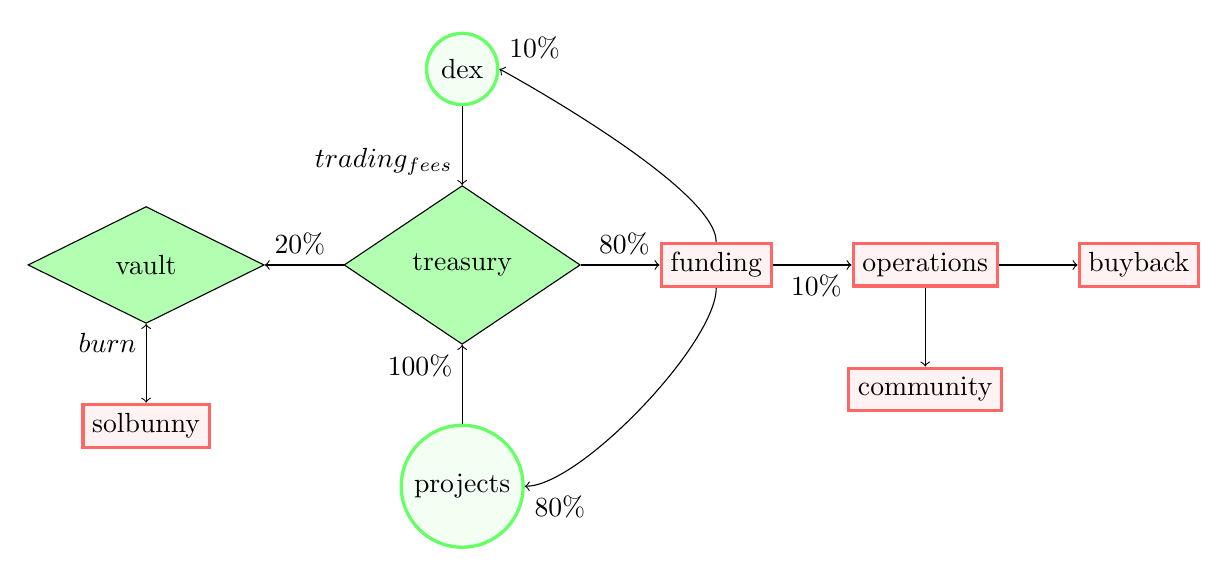
\begin{tikzpicture}[
roundnode/.style={circle, draw=green!60, fill=green!5, very thick, minimum size=7mm},
squarednode/.style={rectangle, draw=red!60, fill=red!5, very thick, minimum size=5mm},
]
%Nodes
\node[decision, yshift=-0.5cm]     (maintopic)                           {treasury};
\node[roundnode]        (uppercircle)       [above=of maintopic] {dex};
\node[squarednode]      (rightsquare)       [right=of maintopic] {funding};
\node[roundnode]        (lowercircle)       [below=of maintopic] {projects};
\node[decision]       (leftsquare)       [left=of maintopic]     {vault};
\node[squarednode]      (rightsquare2)    [right=of rightsquare] {operations};
\node[squarednode]      (leftsquare2)       [below=of leftsquare] {solbunny};
\node[squarednode]      (rightsquare3)    [right=of rightsquare2] {buyback};
\node[squarednode]      (rightlowersquare3)    [below=of rightsquare2] {community};


%Lines
\draw[->] (uppercircle.south) --  (maintopic.north) node[anchor=south east]{$trading_{fees}$};
\draw[->] (maintopic.east) -- (rightsquare.west) node[anchor=south east]{$80\%$};
\draw[->] (rightsquare.south) .. controls +(down:7mm) and +(right:7mm) .. (lowercircle.east) node[anchor=north west]{$80\%$};
\draw[->] (lowercircle.north) -- (maintopic.south) node[anchor=north east]{$100\%$};
\draw[->] (rightsquare.east) -- (rightsquare2.west) node[anchor=north east]{$10\%$};
\draw[->] (maintopic.west) -- (leftsquare.east) node[anchor=south west]{$20\%$};
\draw[<->] (leftsquare2.north) -- (leftsquare.south) node[anchor=north east]{$burn$};
\draw[->] (rightsquare2.east) -- (rightsquare3.west);
\draw[->] (rightsquare2.south) -- (rightlowersquare3.north);
\draw[->] (rightsquare.north) .. controls +(up:7mm) and +(left:0mm) .. (uppercircle.east) node[anchor=south west]{$10\%$};


\end{tikzpicture}


\section*{Calculations}

SolBunny takes advantage of many principles from evolutionary game theory \cite{game} to biochemistry \cite{menten}, but the most important aspect is how tokenomics, as the value proposition for investors, must be preserved through the test of time. The total supply of SolBunny is fixed at\\

1 Quadrillion: 1.000.000.000.000.000 (10\textsuperscript{15}) or 1000 trillion \\

SolBunny is deflationary by default through lost wallets/transactions, but also through planned burns equivalent to 50$\%$ per year. Dormant Bitcoin (never been moved) is currently $\sim$10{\%} \cite{btc} so applying all this to Solbunny, and using the formula for exponential decay \cite{decay}: 


\begin{enumerate}[label=(\roman*)]

\item $N(t)=N_{0}(\frac{1}{2})^\frac{t}{t_{\frac{1}{2}}}$

\item  $N(t)=N_{0}e^{-\frac{t}{\tau}}$

\item  $N(t)=N_{0}e^{-\lambda t}$

\end{enumerate}

$N_{0}$: Initial token supply

$N_{t}$: Remaining quantity after time, t

${t_{\frac{1}{2}}}$: Half-life

$\tau$: Mean lifetime

$\lambda$: Decay constant\\

The ${t_{\frac{1}{2}}}$ can be calculated since only 49$\%$ total supply of SolBunny is left after 1 year:

$N_{0} = 10^{15} SolBunny$\\

\begin{equation}\label{init}
\begin{split}
 N(1) &= 10^{15} - \frac{(10^{15} + 50\cdot 10^{15})}{100}\\
 &= 490^{12} SolBunny
\end{split}
\end{equation}

\begin{equation}\label{decay}
\begin{split}
N(t)&=N_{0}(\frac{1}{2})^\frac{t}{t_{\frac{1}{2}}}\\
490^{12}&=10^{15}(\frac{1}{2})^\frac{1}{t_{\frac{1}{2}}}\\
{t_{\frac{1}{2}}} & = 0,97
\end{split}
\end{equation}
\\

The formula for predicting supply ex-ante:\\

$N(t)=10^{15}(\frac{1}{2})^\frac{t}{0,97}$

\begin{tikzpicture}
  \begin{axis}[ 
    xlabel=$t(years)$,
    xmin=0,
    ylabel={$SolBunny$}
  ] 
    \addplot {(10^(15)) * ((1/2)^(x/0.97))}; 
  \end{axis}
\end{tikzpicture}

However, scarcity does not automatically increase the value of SolBunny—the underlying asset must appreciate in value. The main profit stream will come from trading fees, which depends on how much trading volume SolBunny can realistically capture:

\begin{table}[ht]
\caption{The three largest dex with limit order book system}
\centering
\begin{tabular}{||c c c c||} 
 \hline
Dex & Volume(\$) &  Fee(\%) & Income (\$) \\ [0.5ex] 
 \hline\hline
 Raydium \cite{raydium} & 275M & 0,22 \cite{serum} & 605K \\ 
 \hline
 Dexlab \cite{dexlab} & 120M & 0,22 \cite{dexfee} & 264K \\
 \hline
Mango Markets \cite{mango} & 205M & 0,09 & 94K \\
 \hline
\end{tabular}
\label{Table 1}

Table 1: The three largest dex with limit order book system on a 24-hour basis. The market is highly fragmented beyond these three dex.
\end{table}

Meanwhile, the entire cryptomarket has been growing over 1000x since 2014 \cite{cryptovolume}. The operating costs are estimated to be $\$$2000 per month (maintenance, APIs, improvements, etc). Thus, to break-even with a trading fee of 0,20$\%$:

\begin{equation}\label{break-even}
\begin{split}
break-even &=\frac{trading_{fee}}{100} trading_{volume}\\
\$2000  &=\frac{0,20\%}{100} trading_{volume}\\
trading_{volume} &=\$1M/month\\
 &=\$33K/24-hour
\end{split}
\end{equation}
\\

SolBunny believes this is possible given that a trading volume of \$33K is under 1\% of the top dexes on Solana. In fact, a more realistic trading volume over the first year would be closer to $\sim$\$50M/month so the profits will be:
 
\begin{equation}\label{income by 10x}
\begin{split}
profits &=\frac{trading_{fee}}{100}  \cdot trading_{volume} - costs\\
 &=\frac{0,20\%}{100} \cdot \$50M/month - \$2000/month\\
 &=\$98K/month
\end{split}
\end{equation}
\\


Although this seems prolonged compared to other investments, there are three considerations:

\begin{enumerate}[label=(\roman*)]

\item This is based on the worst-case scenario of consistent growth

\item It is only based on volume, and does not take into account other investments

\item It assumes SolBunny will be burned at a consistent pace (50\% per year)\\

\end{enumerate}


SolBunny will use various DAOs, lend/borrow protocols and leverage to achieve as much profit as possible. SolBunny finds it realistic to hit a CAGR in trading volume of 600\% per year. This growth rate, in addition to the assets appreciating 20\% a year in value projects  at least a decade to achieve ‘essential singularity’ (1 SolBunny =\$1). If the profits grow exponentially then the target will be reached in a few years. SolBunny has deployed several strategies in order to catalyze the reaction towards essential singularity. The major difference between self-perceived value vs. market value is addressed as the market ultimately determines the price of 1 SolBunny. The concept of evolutionary game theory \cite{egt} is a better fit for social systems than traditional game theory, and thus, SolBunny utilizes this fact for three possible scenarios of SolBunny holders:

\begin{table}[ht]
\caption{Game Theory}
\centering
\begin{tabular}{||c| c| c| c||} 
 \hline
Action & Stake &  Burn & Sell \\ [0.5ex] 
 \hline\hline
Stake & (3,3) & (1,3) & (-1,1) \\ 
 \hline
Burn & (3,1) & (1,1) & (-1,1) \\
 \hline
Sell & (1,-1)& (1,-1) & (-3,-3) \\
 \hline
\end{tabular}
\label{Table 2}

Table 2: Traditional view on game theory favoring staking (3,3) as the most rational choice.
\end{table}

Contrary to traditional game theory, these scenarios are not weighted equal in terms of what a normal person or \textit{bonus pater} perceives as rational outcome. In fact, the Nash equilibrium was not a unique solution to the equilibrium selection problem but mixed evolutionarily stable strategies \cite{evogame}.

The general consensus is the following: Good if everyone stakes, ok if someone burns while others stake and bad if everyone sells. However, the situation is far from straightforward for the following reasons:

\begin{enumerate}[label=(\roman*)]

\item Every static situation is merely a snapshot of reality when time is not involved

\item  Rational behavior is based on the individual’s intuition, not the masses

\item  Humans are highly affected in a changing cultural and socio-economic milieu

\end{enumerate}

In table 2, selling is considered detrimental for the protocol but this could not be further from the truth since selling tends to decrease the price of SolBunny, and the protocol can now afford to buy back even more SolBunny for burning. Other investors may buy more SolBunny to burn for a share of the vault, thereby reducing the total supply in circulation. In contrast, staking is not always considered the best strategy as it may inflate the price of SolBunny beyond the capabilities of the protocol’s idle buyback and burn mechanism. In addition, more investors will have to share the vault, and ultimately the treasury chest. The latter will be liquidated over a period of time through staking to eliminate dilution from dead wallets.

SolBunny proposes a revised model for the crypto-industry by introducing: i) A drift, epsilon, in demand over time and ii) A third dimension, t, to determine the changes in drift. In simple terms the entry for each scenario takes a form of: 

$(x+\epsilon, y+ \epsilon, t) \rightarrow (\psi+\epsilon, \psi+ \epsilon, \infty)$

There are no stable equilibrium or static situations, thus only unstable equilibrium is favored and perturbed by $\epsilon$. But SolBunny remains in a favorable position in all scenarios as indicated by $\psi$ (referenced to superposition in quantum physics). \\

tl;dr HODL SolBunny

\clearpage


\section*{Conclusion}

Taken at face value, SolBunny offers three unique value proposition to its members, and can be summarized as follows:

\begin{enumerate}

\item Decentralized protocol: Each member owns their own liquidity without any focal points, and will be able to move freely between all platforms. They may even fork a new project from the main branch to start their own

\item Market agnostic value: The value of SolBunny will increase, regardless of sentiment in crypto as the tokenomics, dex and launchpad are independent of price or exit liquidity

\item Real-world utility: The closed loop of funding real-world projects to generate profits provides value beyond crypto, and makes SolBunny intra-diversified by default

\end{enumerate}

tl:dr SolBunny wants to create a stock exchange, like NYSE or Nasdaq, governed by the people of its community.


\clearpage

\section*{Acknowledgments}
The authors are all active in Discord, and would like to thank all the members of SolBunny. A special thanks goes to the regular moderators who are performing daily miracles. Lastly, Gerald Hefner (aka. supreme leader) and GRACKATTACK has provided valuable input to our discussions. They were truly an inspiration for this article as well as everyone else in the community.


\bibliography{scibib}

\bibliographystyle{Science}



\clearpage

\section*{Supplementary}
The compounded annual growth (CAGR) of the cryptomarket is:

\begin{equation}\label{growth}
\begin{split}
CAGR^{2014-2021} &= \frac{t_{1}}{t_{0}}^{\frac{1}{n}}-1\\
 &=  (\frac{\$100B}{\$72M})^{\frac{1}{7}}-1\\
 &=185\%
\end{split}
\end{equation}
\\

Applying these numbers to SolBunny to determine future growth:

\begin{equation}\label{growth}
\begin{split}
y &=ax+b\\
income &=\frac{185\%}{100}\$98K/month \cdot 12months \cdot x + \$98K/month \cdot 12months\\
 &= \$2,1M \cdot x + \$1,1M
\end{split}
\end{equation}
\\

However, the costs are also expected to increase over time though not as fast as income. Assuming a 25\% annual increase in maintenance costs:

$\$2000*12months*1,25=\$30K/year$

Thus, the linear growth is expected to generate following profits:

\begin{equation}\label{profits}
\begin{split}
y &=ax+b\\
profits &=(income-costs) \cdot x + (income-costs)\\
 &= (1,85 \cdot \$100K/month - \$2000 \cdot 1,25)\cdot 12months \cdot  x + (\$100K/month - \$2000 \cdot 1,25)\cdot 12months\\
 &= \$2,1M \cdot x + \$1,1M
\end{split}
\end{equation}
\\

Given the scarcity of SolBunny and accruing value of its underlying asset:

\begin{equation}\label{target}
\begin{split}
N(t) &=10^{15}(\frac{1}{2})^\frac{t}{0,97}\\
profits(t) &=N(t)\\
\$591K \cdot t+ \$306K&=10^{15}(\frac{1}{2})^\frac{t}{0,97}\\
0 &=10^{15}(\frac{1}{2})^\frac{t}{0,97}-\$2,1M \cdot t-\$1,1M\\
t &= 23years
\end{split}
\end{equation}
\\

t=$\sim$23 years for 1 SolBunny = \$1\\
SolBunny introduces a new method, ‘quantum-hop’, for the market to determine its price. Essentially, quantum-hop is the ability for holders to burn their tokens for a proportion of the vault, and the vault takes 20\% of the profits \textit{pro bene}. In addition, SolBunny metaDAO possesses the majority of SolBunny so an even larger burn is possible if its community decides to do so. If 99\% of SolBunny is burned within the first year and 25\% more each year ($t_{\frac{1}{2}}=0,69$) while SolBunny dex outpaces the general market to hit a CAGR in trading volume of 600\% per year (3x):

\begin{equation}\label{2x}
\begin{split}
0 &=10^{13}(\frac{1}{2})^\frac{t}{0,69} - 2 \cdot \$6,3M \cdot t-\$1,1M\\
 &= 12years
\end{split}
\end{equation}
\\

For every incremental 10x in profits the treasure chest manages to capture every year, the time for SolBunny = \$1 reduces by roughly 2 years. For example, 10x profits:

\begin{equation}\label{10x}
\begin{split}
0 &=10^{13}(\frac{1}{2})^\frac{t}{0,69} - 20 \cdot \$63M \cdot t-\$1,1M\\
&= 10years
\end{split}
\end{equation}
\\
The market price of SolBunny is expected to be at or higher than the value retrieved from the vault by burning SolBunny. As such, investors are being offered a premium to leave the protocol at any time or hold long-term for mutually exclusive and collectively exhaustive benefits of the protocol. The latter also involves liquidation of the treasury chest, and only possible through a vote. Thus, the pricing-strategy of 1 SolBunny approaches the principle of something between a European option (treasury chest) and an American option. European options can only be exercised on its maturity date while American options can be exercised at any time.

Black-scholes formula \cite{bscholes} is often used to predict the fair value of European options according to [option value] = [Intrinsic value] + [Time value]. In contrast, the binomial tree can be used to value both European and American options although only the latter will be considered with the two-step binomial tree with 20\% volatility:


\begin{equation}\label{black}
\begin{split}
f &=e^{-r(t_{1} -t_{0})} \cdot [\frac{e^{r(t_{2} - t_{1})}-d}{(u-d)} \cdot f_{u} + (1-\frac{e^{r(t_{2} - t_{1})}-d}{(u-d)}) \cdot f_{d}]\\
 &= e^{-0,05(1 - 0)} \cdot [\frac{e^{0,05(1 - 0)}-0,25\cdot10^{-8}}{(1,2-0,8)} \cdot 2,83\cdot10^{-9} + (1-\frac{e^{0,05(1 - 0)}-0,25\cdot10^{-8}}{(1,2-0,8)}) \cdot 7,12\cdot10^{-9}]\\
  &=e^{-0,05(1 - 0)} \cdot [0,628 \cdot 2,83\cdot10^{-9} + (1-0,628) \cdot 7,12\cdot10^{-9}]\\
 &=4,21\cdot10^{-9}
\end{split}
\end{equation}
\\

$f$: derivative value at time zero,
$f_{u}$: derivative at node up,
$f_{d}$: derivative at node down,
$r$: Risk-free rate,
$t$: Time to maturity,
$d$: 1+ the percentage move of the SolBunny to reach the downside scenario price,
$u$:  1+ the percentage move of the SolBunny to reach the upside scenario price,
$S_{ou}$: underlying price at node up,
$S_{od}$: under price at node down\\

Thus, the market value of SolBunny is priced at $\$7,12*10^{-9}$ and buying power is expected to outweigh the selling pressure below this threshold. Also, the protocol itself will initiate a strong buyback and burn below the threshold using the Michaelis-Menten formula \cite{mm}:

\begin{equation}\label{mm}
[Buyback/burn]=[Max (buyback/burn)] * \$BUNNY/ (\$BUNNY+ \$SOL/\$10^{12})
\end{equation}\label{mm}

The lower the price of Solbunny drops below the threshold, the more SolBunny will buy back and burn until equilibrium is established.This auto-regulative ability of the protocol is named ‘organic period-doubling bifurcation in situ metamorphosis’ (OPBISM) or just rebase.

SolBunny aims to add as many nodes as possible, and each node will be sub-1-second to approximate real-time SolBunny movements with great accuracy. As the number of nodes increases, the binomial distribution approaches the lognormal distribution assumed by Black-Scholes. The heavy deflationary mechanisms from the protocol may approximate active holders to a logistic map \cite{logmap}:

\begin{equation}\label{mm}
x_{n+1} =rx_{n}(1-x_{n})
\end{equation}\label{mm}

$r$: Growth rate, $x$: Theoretical max between 0 and 1

What is seen from iterations of the logistic map is how the equilibrium number of active holders is independent of the initial number of holders. Thus, the equilibrium will depend solely on r, and if r<1 the number of active holders will go extinct. This is a detrimental scenario that can unfold when not enough voters are able to liquidate the treasure chest because a certain quorum is not met. To counter this, SolBunny implemented a timer on the treasure chest to self-release its assets to stakers over the course of one week on 5 November 2031. More exactly, the theoretical time it will take SolBunny to hit essential singularity while the growth of active holders (r) stays at 2 and the theoretical max of active holders (x) is 0,1 \textperthousand.





\end{document}




















